\section*{Теория}

\textit{Эффектом Поккельса} называется изменение показателя преломления света в кристалле под действием электрического поля, причём
это изменение пропорционально напряжённости электрического поля.
Вследствие эффекта Поккельса в кристалле необата лития одноосный кристалл становится двуосным.

Изменение показателя преломления кристаллов под действием
внешнего электрического поля происходит за счёт анизотропных
свойств кристаллов. Под действием постоянного электрического поля
электроны смещаются в сторону того или иного иона (в случае
кристалла ниобата лития LiNbO$_3$ — это ион Li или Nb), при этом
меняется поляризуемость среды и связанный с ней показатель преломления. Эффект Поккельса может наблюдаться только в кристаллах, не обладающих центром симметрии. Кристалл можно поместить между двумя скрещенными
поляроидами таким образом, что в отсутствие внешнего электрического поля пропускание света системой будет равно нулю. При подаче
на кристалл внешнего поля появится наведённое двулучепреломление,
которое изменит поляризацию прошедшего через кристалл света, и
такая система начнёт пропускать свет.

\begin{figure}[H]
	\centering
	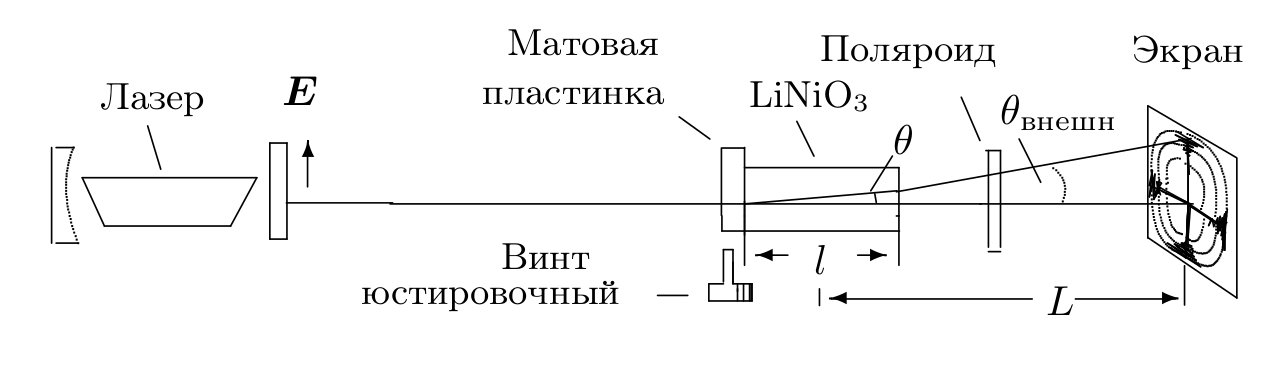
\includegraphics[width=0.8\textwidth]{../Изображения/scheme1.png}
	\caption{Схема наблюдения эффекта Поккельса}
\end{figure}

Рассмотрим сначала кристалл в отсутствие внешнего электрического поля. Кристалл ниобата лития является одноосным кристаллом, то
есть кристаллом, оптические свойства которого обладают симметрией
вращения относительно некоторого одного направления, называемого
оптической осью $z$ кристалла.

Для световой волны, вектор электрического поля $\boldsymbol{E}$ которой перпендикулярен оси $z$, показатель преломления равен $n_o = \sqrt{\varepsilon_\perp}$, а для волны, вектор $\boldsymbol{E}$ которой располагается вдоль оси $z$, он равен $n_E = \sqrt{\varepsilon_{||}}$, причём $n_e < n_o$.

Если луч света распространяется под углом $\theta$ к оптической оси $z$, то существуют два собственных значения показателя преломления $n_1$ и $n_2$. Если световой вектор перпендикулярен плоскости ($\boldsymbol{k}$, $\boldsymbol{e_z}$), то для обыкновенной волны $n_1 = n_o$.  Если световой вектор лежит в плоскости ($\boldsymbol{k}$, $\boldsymbol{e_z}$), то для необыкновенной волны $n_2$ зависит от угла $\theta$ и определяется формулой:
$$
\frac{1}{n_2^2} = \frac{\cos^2 \theta}{n_o^2} + \frac{\sin^2 \theta}{n_e^2}
$$

Если перед кристаллом, помещённым между скрещенными поляроидами, расположить матовую пластинку, после которой лучи будут рассеиваться под различными углами, то на экране, расположенном за поляроидом, будут наблюдаться тёмные концентрические окружности (коноскопическая картина) -- результат интерференции обыкновенной и необыкновенной волн.

Разность фаз между обыкновенной и необыкновенной волнами, при-
обретаемая при прохождении через кристалл длиной $l$, равна
$$
\Delta \varphi = \frac{2 \pi}{\lambda} \cdot l \cdot (n_1 - n_2)
$$

Считая, что $n_o - n_e \ll 1$, а углы малые $\theta \ll 1$, получаем
$$
n_2 \approx n_o - (n_o - n_e) \theta^2
$$
Итоговая формула для набега фазы:
$$
\Delta \varphi = \frac{2 \pi}{\lambda} l (n_o - n_e) \theta^2
$$
Направлениями постоянной разности фаз служат конусы $\theta = const$,
поэтому интерференционная картина представляет собой концентрические окружности. Интерференционные кольца перекрываются тёмным крестом, который выделяет области, где интерференция отсутствует. В этих направлениях распространяется только одна поляризованная волна. При повороте анализатора на $90^\circ$ картина меняется с позитива на негатив.

Для случая, когда разрешённое направление анализатора перпендикулярно поляризации лазерного излучения определим радиус тёмного кольца с номером $m$. Для луча, идущего вдоль оси $z$, показатели преломления для двух волн совпадают, сдвиг фаз между ними равен нулю, поляризация излучения на выходе остаётся такой же, как на входе, и луч не проходит через анализатор. Картина не изменится при сдвиге фаз между обыкновенной и необыкновенной волной, кратном $2\pi$. $\Delta \varphi = 2 \pi m$. Пусть $L$ -- расстояние от центра кристалла до экрана. По закону Снеллиуса, на на границе кристалла луч света преломляется и $\theta_{внеш} = n_0 \theta$. Радиус тёмных колец определяется по формуле: \\
$$
r_m^2 = \frac{\lambda}{l} \frac{(n_o L)^2}{(n_o - n_e)} m
$$

\begin{wrapfigure}{l}{0.3 \textwidth}
	\centering
	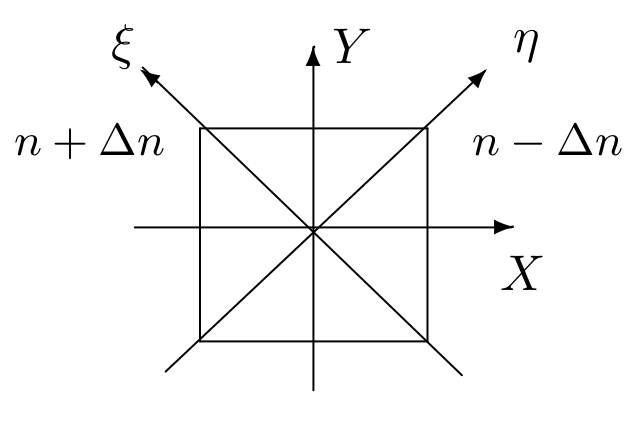
\includegraphics[width=0.28\textwidth]{../Изображения/scheme2.png}
	\caption{Главные направления в кристалле во внешнем электрическом поле}
\end{wrapfigure}

Если поместить кристалл во внешнее электрическое поле, то из-за симметрии кристалла и его электрических свойств в плоскости xy появляются главные направления $\xi$ и $\eta$ с показателями преломления $n_o - \Delta n$ и 
$n_o + \Delta n$. Изменение показателя преломления линейно связано со значением внешнего электрического поля $\Delta n = A \cdot E_{эл}$.

После прохождения кристалла между обыкновенной и необыкновенной волнами появляется разность фаз: \\
$$
\Delta \varphi = \frac{4 \pi}{\lambda} \frac{l}{d} AU
$$
где $U = E_{эл} d$ -- напряжение на кристалле, $d$ -- размер кристалла в поперечном направлении. 

Результирующее поле после анализатора определяется выражением: \\
$$
E_{вых} = E_0 e^{i(\omega t - k l)} \sin \left(\frac{\Delta \varphi}{2}\right)
$$

Интенсивность света на экране определяется по формуле: \\
$$
I_{вых} = I_0 \sin^2 \left( \frac{\pi}{2} \frac{U}{U_{\frac{\lambda}{2}}} \right)
$$
где $U_{\frac{\lambda}{2}} = \frac{\lambda}{4A} \frac{d}{l}$ -- полуволновое напряжение.

Если разрешённые направления пропускания лазера и анализатора будут параллельны, то интенсивность будет определяться по формуле: \\
$$
I_{вых} = I_0 \cos^2 \left( \frac{\pi}{2} \frac{U}{U_{\frac{\lambda}{2}}} \right)
$$